% !TEX TS-program = xelatex
% !TEX encoding = UTF-8 Unicode
% !Mode:: "TeX:UTF-8"

\documentclass{resume}
\usepackage{zh_CN-Adobefonts_external} % Simplified Chinese Support using external fonts (./fonts/zh_CN-Adobe/)
%\usepackage{zh_CN-Adobefonts_internal} % Simplified Chinese Support using system fonts
\usepackage{linespacing_fix} % disable extra space before next section
\usepackage{cite}
\usepackage{graphicx}
\usepackage{tabu}
\usepackage{multirow}
\usepackage{color}
\usepackage{hyperref}
\begin{document}
\pagenumbering{gobble} % suppress displaying page number

\Large{
  \begin{tabu}{ c l r }
   \multirow{5}{1in}{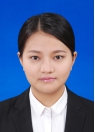
\includegraphics[width=0.88in]{ct-1inch}} & \scshape{陈天} & \pbar{Python}{0.7} \\
    & \email{tianchenucas@gmail.com} & \pbar{C/C++}{0.5} \\
    & \phone{(+86) 188-102-15921} & \pbar{Linux}{0.6} \\
    & \github[github.com/clovischen]{https://github.com/clovischen} & \pbar{ROS}{0.5}\\
    ~~
  \end{tabu}
}

% \Large{
%   \begin{tabu}{ c l r }
%    \multirow{5}{1in}{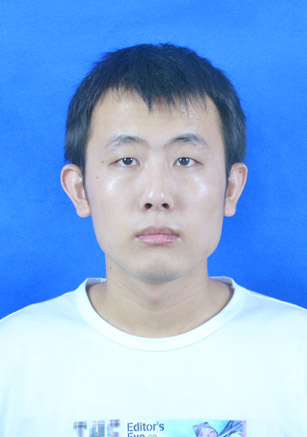
\includegraphics[width=0.88in]{DSC_0804}} & \scshape{陈天} & \pbar{Python}{0.7} \\
%     & \email{tianchenucas@gmail.com} & \pbar{Python}{C/C++0.5} \\
%     & \phone{(+86) 188-102-15921} & \pbar{Linux}{0.6} \\
%     & \linkedin[boin]{https://www.linkedin.com/in/bobin-ding-55496b134/} & \pbar{ROS}{0.5} \\
%     & \github[github.com/clovis]{https://github.com/clovis} & \pbar{QT}{0.5}
%   \end{tabu}
% }


\section{\faGraduationCap\  教育背景}
\datedsubsection{\textbf{中国科学院自动化研究所}, 北京}{\textit{在读硕士} \quad 控制理论与控制工程 \quad 2016 -- 至今}
\datedsubsection{\textbf{北京邮电大学}, 北京}{\textit{工学学士}\qquad 电子科学与技术 \quad 2012 -- 2016}

\section{\faUsers\ 项目经历}
\datedsubsection{\textbf{基于卡尔曼滤波器的跟踪器}}{\quad 2017.01 - 2017.05}
\begin{itemize}\small
  \item 针对视频
  \item
\end{itemize}

\datedsubsection{\textbf{谱聚类}}{\quad 2016.12 -- 2016.01}
\begin{itemize}\small
  \item ???
  \item ????????
\end{itemize}

\datedsubsection{\textbf{新闻检索}}{ \quad 2016.09 -- 2016.12}
\begin{itemize}\small
  \item 新闻检索系统使用爬虫抓取新闻预料。
  \item 
\end{itemize}

\datedsubsection{\textbf{自闭症辅助医疗机器人交互系统}}{ \quad 2016.03 -- 2016.06}
\begin{itemize}\small
  \item 针对自闭症患者设计医疗机器人交互系统,其中情绪监控单元使用AdaBoost对人脸表情进行分类。
  \item 基于典型的特教训练任务完成交互系统以及可视化仿真。
\end{itemize}


\datedsubsection{\textbf{基于红外传感器的避障小车}}{ \quad 2015.03 -- 2015.06}
\begin{itemize}\small
  \item
  \item
\end{itemize}

\section{\faCogs\ 技能}
% increase linespacing [parsep=0.5ex]
\begin{itemize}\small
\item 熟练Linux下常用指令及C++,Python,ROS开发环境。
\item 理解常用的视觉(惯性)SLAM/VO算法(SVO,DSO,ORB SLAM)。
\item 熟悉常用的结构设计工具 Solidworks,AutoCAD,NX,ANSY。
\item 熟悉常用的SLAM工具 (Sophus、Eigen、G2O),熟练使用OpenCV。
\end{itemize}

\section{\faHeartO\ 获奖情况}

\vbox{{\small
  \begin{tabular}{l l}
本科阶段 & 北京邮电大学英语风采大赛团体二等奖\\
  \end{tabular}
}}


 % \section{\faInfo\ 自我评价}{\small
 %  % increase linespacing [parsep=0.5ex]
 % \begin{itemize}[parsep=0.5ex]
 %  \item 态度端正,善于思考 ;学习勤奋,积极向上 ;性格开朗,热爱生活 。
 % \end{itemize}
 % }

%% Reference
%\newpage
%\bibliographystyle{IEEETran}
%\bibliography{mycite}
\end{document}
